\atstartofhistorysection
\section[Un peu d’histoire : le rêve de Rudolf Diesel]{Un peu d’histoire :\onlyamphibook{\\} le rêve de Rudolf Diesel}
\label{ch_histoire_diesel}\index{Diesel!Rudolf|(textbf}

	C’est l’histoire d’un moteur né dans la marge d’un cours de thermodynamique. «~\textit{Kann man Dampfmaschinen konstruieren, welche den vollkommenen Kreisprozess ausführen, ohne zu sehr kompliziert zu sein?}~» : peut-on construire des machines à vapeur capables d’effectuer le cycle idéal sans être trop complexes ? L’étudiant \mbox{Rudolf} Diesel se pose la question en marge de ses notes en 1878 à Munich, ayant réalisé que le cycle moteur suivi par les machines à vapeur de son époque les condamne irrémédiablement à des rendements médiocres.

	\index{isothermes, évolutions}\index{évolutions!isothermes}\index{injection directe}
	Ainsi va mûrir au fil des années le concept d’un \textit{moteur à chaleur rationnel}, dont les caractéristiques seront finalement publiées en 1893~\cite{diesel1893, diesel1893en}. Rudolf Diesel est sans équivoque : «~un examen de leur théorie de fonctionnement montrera que les moteurs à gaz et à air fonctionnent sur la base d’un principe défectueux, et aucune amélioration ne produira de meilleurs résultats tant que ce principe est retenu~». Il n’est pas plus tendre avec les concepteurs des moteurs à vapeur.\\
	Les principaux traits du moteur proposé découlent strictement de préceptes physiques : il s’agit de s’approcher au plus près du cycle de Carnot, en «~\textit{produi[sant] la température la plus haute du cycle (la température de combustion) non pas par et pendant la combustion, mais avant et indépendamment d’elle, entièrement par la compression d’air ordinaire}~». S’en suit une combustion à température constante, contrôlée par injection progressive de carburant. Seules la vidange et l’admission (effectuées à pression constante avec un cycle à quatre temps) s’éloignent du cycle de Carnot.
	
	\begin{figure}
		\begin{center}
			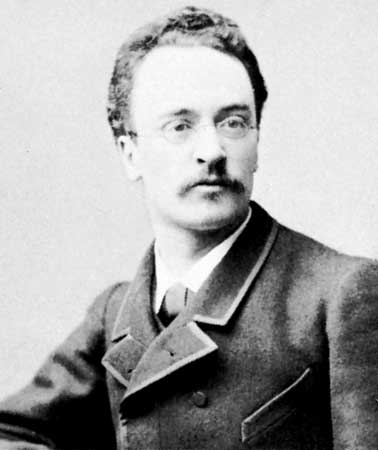
\includegraphics[width=5cm]{images/rudolf_diesel_1883.jpg}
		\end{center}
		\supercaption{Rudolf Diesel en 1883.}{\wcfile{Diesel 1883.jpg}{photo} d’auteur inconnu (\pd)}
		\label{fig_rudolf_diesel}
	\end{figure}
	
	\index{auto-inflammation}\index{combustible!auto-inflammation}\index{injection directe}
	Les caractéristiques annoncées sur le papier donnent à réfléchir : la pression maximale de compression doit être au moins de $p_2 = p_1 \left( \frac{T_\text{combustion}}{T_\text{initiale}} \right)^{\frac{\gamma}{\gamma -1}}$ (\ref{eq_isentropique_horrible2}), ce qui mène Rudolf Diesel~à \SI{300}{\bar} -- vingt fois plus que les moteurs existants ! Le concept de l’injection directe, que les hautes températures atteintes pendant la compression rendent nécessaire afin d’éviter une combustion prématurée, est convaincant. Toutefois, il manque bien des détails sur la manipulation de la poudre de charbon --\ carburant choisi par Rudolf Diesel pour son abondance et son faible coût\ -- qui permettra en pratique son injection directe dans les cylindres.

	\index{pression!maximale d’un moteur}\index{moteur!pression maximale d’un}
	Malgré tout, Rudolf Diesel, après un début de carrière remarqué dans la conception de systèmes de réfrigération, réussit à convaincre l’entreprise \textit{Maschinenfabrik Augsburg-Nürnberg}, connue aujourd’hui sous le nom de \textsc{man}, de financer ses recherches. Elles seront difficiles : le passage de la théorie à la pratique pendra quatre ans. Beaucoup d’ambitions sont revues à la baisse : la pression maximale descend à~\num{90} puis~\SI{40}{\bar}, la poudre de charbon est abandonnée au profit d’une huile peu raffinée de manipulation plus simple. Comme ce sont les limites structurelles du moteur qui contraignent le cycle, la combustion isotherme est remplacée par une isobare à pression maximale. Le second prototype, un mono-cylindre de près de trois mètres de hauteur (\cref{fig_diesel_second_prototype}), est le premier à fonctionner de façon autonome : huit minutes en février 1894. Les performances du troisième prototype (\cref{fig_diesel_third_prototype})	seront mesurées indépendamment en 1897 : \SI{17}{ch} à \SI{154}{rpm}, et un rendement de~\SI{26,2}{\percent}. Cette efficacité était deux fois supérieure à celle de ses contemporains à combustion interne, et quatre fois supérieure à celle des meilleurs moteurs à vapeur !
	\begin{figure}
		\begin{center}
			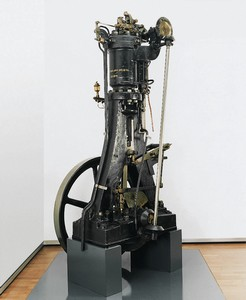
\includegraphics[width=6cm]{images/diesel_second_prototype.jpg}
		\end{center}
		\supercaption{Le second prototype développé chez \textsc{man} par Rudolf Diesel, et le premier à fonctionner de façon autonome, en février 1894. Il n’y a qu’un cylindre de \SI{22}{\centi\metre} de diamètre, et l’injection directe de carburant se fait par un circuit d’air comprimé. Le moteur est aujourd’hui exposé au siège de l’entreprise \textsc{man}.}%
		{\wcfile{First Diesel.jpg}{photo} \ccbysa MAN SE}
		\label{fig_diesel_second_prototype}
	\end{figure}
	\begin{figure}
		\begin{center}
			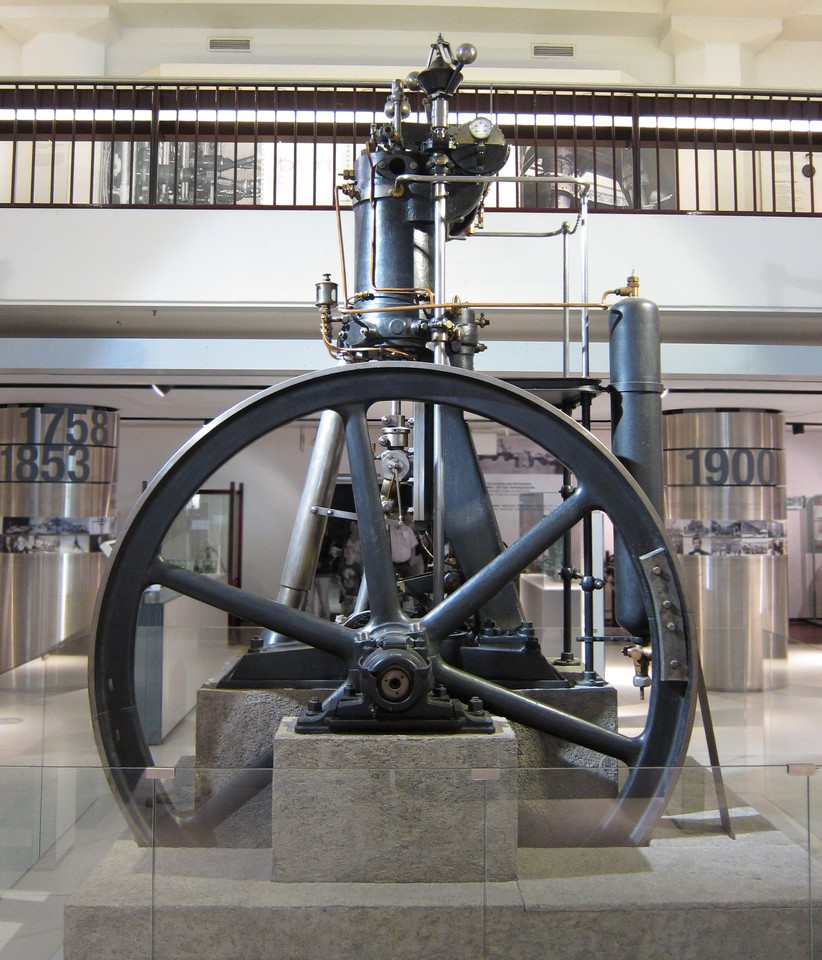
\includegraphics[width=8cm]{images/diesel_third_prototype.jpg}
		\end{center}
		\supercaption{Le troisième prototype de Diesel, et le premier moteur opérationnel. La course du cylindre de \SI{25}{\centi\metre} de diamètre atteint \SI{40}{\centi\metre}. Il sera mis sur banc d’essai à l’université technique de Munich où il atteindra \SI{26,2}{\percent} d’efficacité en 1897. Il est exposé au \textit{Deutsches Museum}.}%
		{\wcfile{Historical Diesel engine in Deutsches Museum.jpg}{photo} \ccbysa \olivier}
		\label{fig_diesel_third_prototype}
	\end{figure}
	
	\index{Diesel!moteur}
	\textsc{Man} met rapidement en vente le \textit{moteur rationnel}, rebaptisé \textit{Diesel}, qui connaîtra un succès progressif en Europe. Sa régularité en fonctionnement, sa fiabilité et surtout sa faible consommation justifient son important coût d’achat : à cause des matériaux et de la précision de fabrication qu’il requiert, son prix par \si{watt} de puissance est environ trois fois supérieur à ses concurrents. Les brevets déposés par Rudolf Diesel lui assurent un revenu important.
	
	Les nombreux documents laissés derrière lui font de Diesel un personnage attachant : cultivé, appliqué et intelligent (il majore toutes ses promotions), il a un ressenti très fin des bouleversements économiques et sociaux provoqués par la mécanisation rapide de l’industrie et des transports à la fin du \textsc{xix}\ieme siècle~\cite{grosser1978,thomas1978,coltrane1997}. Après une enfance rude et misérable, chassé de France puis d’Angleterre, il nourrit un fort idéal social qui le mènera à écrire \textit{Solidarismus} («~\textit{le salut rationnel et économique de l’humanité}~», 1903~\cite{diesel1903}). Pour lui, la décentralisation de la production de puissance mécanique, pour les petites entreprises ou collectifs par exemple, constituerait une avancée sociale déterminante.
	
	En dépit du succès remarquable rencontré en quinze années, Rudolf Diesel peine à trouver l’épanouissement. Il sera constamment la cible de conflits juridiques, ses critiques et concurrents avançant --\ sans avoir tout à fait tort\ -- que les moteurs qu’il commercialise sont finalement très éloignés de la machine décrite dans son brevet. Les montées nationalistes préalables au déclenchement de la première guerre mondiale l’ébranlent. Piètre gestionnaire financier, il multiplie les dépenses déraisonnables et les investissements ruineux et, surtout, il est accablé de fortes migraines et de problèmes médicaux. En 1913 l’homme semble torturé par ses propres questionnements éthiques et philosophiques. Ses moteurs produisent exclusivement de la puissance dans les usines et les centrales électriques : contribuent-ils finalement à l’émancipation ou au maintien des classes ouvrières ? Il met fin à sa vie en septembre.
	
	\begin{figure}
		\begin{center}
			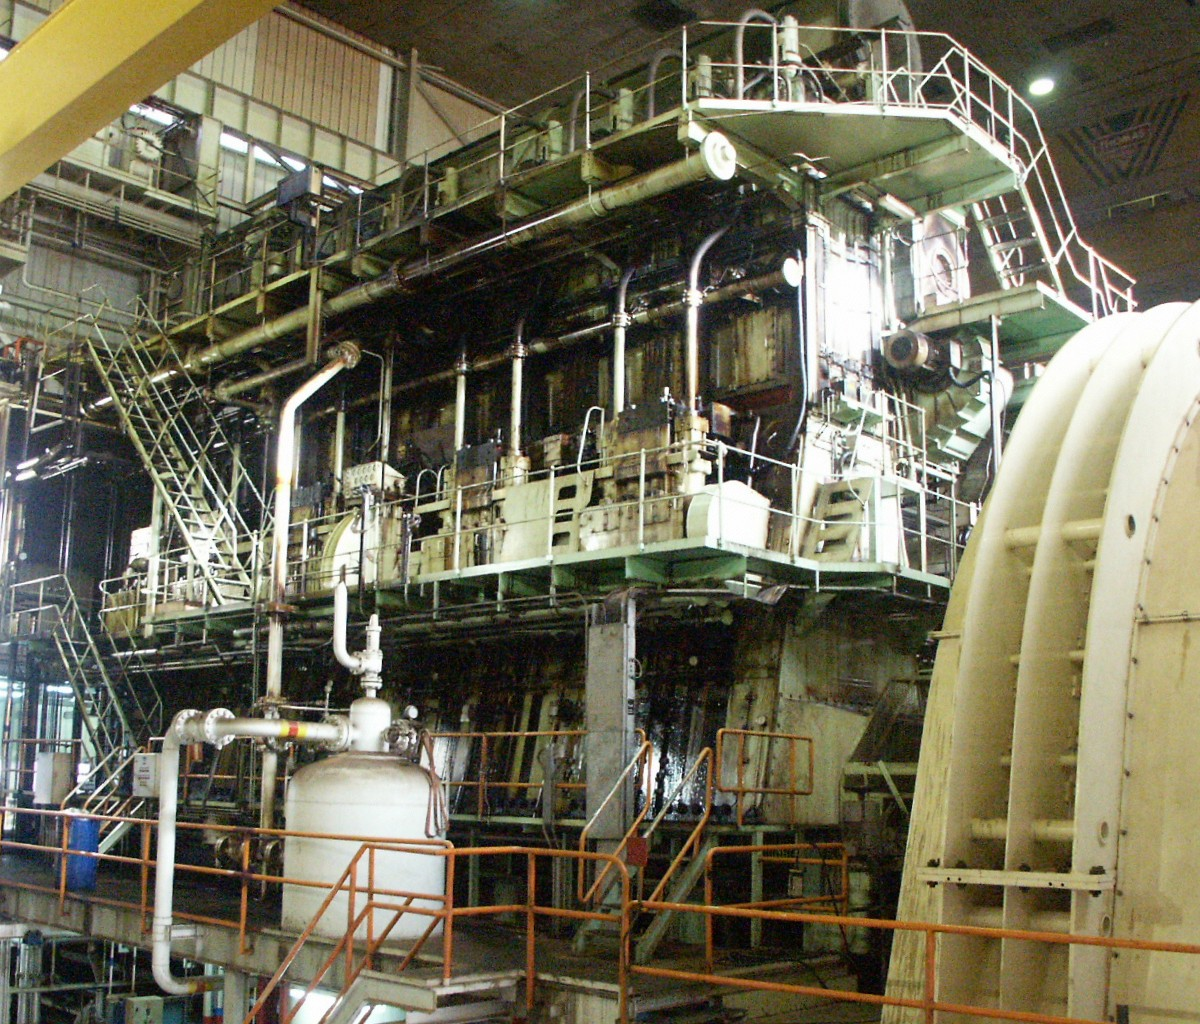
\includegraphics[width=8.5cm]{images/diesel_sulzer_rta76.jpg}
		\end{center}
		\supercaption{Un moteur Diesel \textit{Sulzer RTA76} à neuf cylindres dégageant \SI{25}{\mega\watt} de puissance à \SI{95}{rpm}. Cet exemplaire est installé ici dans une usine mais le modèle est couramment utilisé pour propulser des navires marchands.}{\wcfile{SULZER 9RTA76.JPG}{photo} \ccbysa par \wdu{Sleipnir}}
		\label{fig_sulzer_rta76}
	\end{figure}
	La disparition tragique de son concepteur ne suffira pas à ralentir la progression du moteur Diesel. Les obstacles technologiques à son adoption dans les transports, en particulier le délicat système d’injection du carburant, sont surmontés un à un. Aujourd’hui, il est utilisé partout où les contraintes d’économie et de durabilité priment sur la légèreté et la réactivité.\\
	Dans les navires marchands, des moteurs Diesel hauts de plusieurs étages fonctionnent selon des cycles à deux temps fortement turbocompressés. Dans ces moteurs dépassant \SI{2000}{\tonne} et \SI{18 000}{ch} (\cref{fig_sulzer_rta76}),	les cylindres glissent lentement sur des courses de plus de deux mètres, permettant une combustion quasi-isotherme à~\SI{80}{rpm} et une efficacité dépassant~\SI{50}{\percent}.\\
	À l’autre extrémité du spectre, les Diesels propulsant les plus petits véhicules utilitaires bénéficient de nombreux systèmes permettant d’augmenter leur réactivité et d’étendre leurs gammes de puissance et de couple. Dans ces minuscules machines de~\SI{80}{ch} tournant au delà de \SI{2000}{rpm}, les systèmes électroniques de contrôle effectuent jusqu’à quatre injections de carburant à~\SI{2000}{\bar} directement dans le cylindre pour chaque combustion, optimisant la combustion en fonction de la puissance demandée~\cite{bosch2005}.
	
	Au final, il n’est probablement pas un produit de l’industrie que nous ne fabriquions aujourd’hui dont les matériaux ou composants n’aient été puisés, assemblés et transportés sans l’apport de puissance d’un moteur Diesel. Un bel accomplissement pour un étudiant curieux !

\index{Diesel!Rudolf|)textbf}
\atendofhistorysection
